\documentclass[tikz,border=10pt]{standalone}
\usepackage{amsmath}
\usetikzlibrary{arrows.meta, positioning, calc, decorations.pathreplacing}
\definecolor{c1}{HTML}{000000}
\definecolor{c2}{HTML}{233D4D}
\definecolor{c3}{HTML}{FE7F2D}
\definecolor{c4}{HTML}{EAECF0}
\definecolor{axiscolor}{HTML}{333333}
\definecolor{labelcolor}{HTML}{5F6B75}
\begin{document}
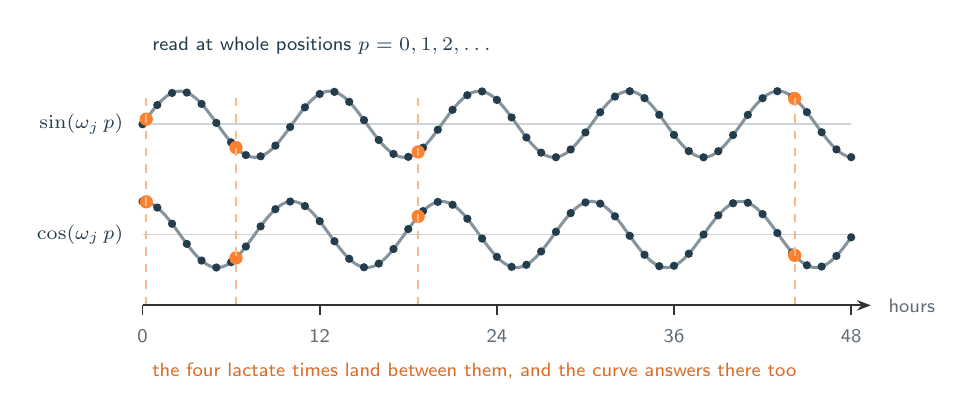
\begin{tikzpicture}[
    every node/.style={font=\sffamily},
    lab/.style={font=\sffamily\scriptsize, text=labelcolor},
    tag/.style={font=\sffamily\scriptsize, text=c2},
    hot/.style={font=\sffamily\scriptsize, text=c3!85!black},
]
\def\X#1{1.70 + #1*0.1875}

% two coordinates of one pair
\foreach \y/\f/\name in {4.55/0.62/{$\sin(\omega_j\, p)$}, 3.15/0.62/{$\cos(\omega_j\, p)$}}{
    \draw[c2!22, line width=0.6pt] (1.70, \y) -- (10.70, \y);
    \node[tag, anchor=east] at (1.58, \y) {\name};
}
\draw[c2!55, line width=1.1pt]
    plot[domain=0:48, samples=240, smooth] ({\X{\x}}, {4.55 + 0.42*sin((\x*0.62) r)});
\draw[c2!55, line width=1.1pt]
    plot[domain=0:48, samples=240, smooth] ({\X{\x}}, {3.15 + 0.42*cos((\x*0.62) r)});

% what we have been reading: whole positions only
\foreach \p in {0,1,...,48}{
    \fill[c2] ({\X{\p}}, {4.55 + 0.42*sin((\p*0.62) r)}) circle (1.5pt);
    \fill[c2] ({\X{\p}}, {3.15 + 0.42*cos((\p*0.62) r)}) circle (1.5pt);
}
\node[tag, anchor=west] at (1.70, 5.55) {read at whole positions $p = 0, 1, 2, \dots$};

% what the formula will answer just as well
\foreach \t in {0.25, 6.33, 18.67, 44.17}{
    \fill[c3] ({\X{\t}}, {4.55 + 0.42*sin((\t*0.62) r)}) circle (2.4pt);
    \fill[c3] ({\X{\t}}, {3.15 + 0.42*cos((\t*0.62) r)}) circle (2.4pt);
    \draw[c3!55, line width=0.7pt, dashed] ({\X{\t}}, 2.25) -- ({\X{\t}}, 4.97);
}
\node[hot, anchor=west] at (1.70, 1.42)
    {the four lactate times land between them, and the curve answers there too};

\draw[axiscolor, line width=0.8pt, -{Stealth[length=5pt]}] (1.70, 2.25) -- (10.95, 2.25);
\foreach \p in {0, 12, 24, 36, 48}{
    \draw[axiscolor, line width=0.7pt] ({\X{\p}}, 2.25) -- ({\X{\p}}, 2.13);
    \node[lab, anchor=north] at ({\X{\p}}, 2.07) {\p};
}
\node[lab, anchor=west] at (11.05, 2.25) {hours};
\end{tikzpicture}
\end{document}
